% Cote 119: offprints, reports, courses, CV and letters (typed and printed part): archive cote 119, site page 168 (PDF page 169).
% typescript. Draft compared: none.
% AI-transcribed by Claude Opus 5.5 (claude-opus-5-5, adaptive thinking, effort high), Message Batches API, batch r119_full (msgbatch_01DwZNm5Y7YsKBWyAN4sFs8w), 2026-11-13; not yet checked by eye.
\scanpage{119/168}
\mspage{- 7 -}

\uline{Définition 3.5.}
On dit qu'une forme différentielle $\omega$ à coefficients $P$ et $Q$
continus dans un ouvert $U$ est fermée si tout point $(x_o,y_o) \in U$ possède
un voisinage ouvert dans lequel $\omega$ a une primitive. On a alors la :

\uline{Proposition 3.6.}

Pour qu'une forme différentielle $\omega$ dans un ouvert $U$ soit fermée
il faut et il suffit que l'on ait $\int_\gamma \omega = 0$ chaque fois que $\gamma$ est le bord
d'un rectangle contenu (ainsi que son intérieur) dans $U$ et ayant ses côtés
parallèles aux axes.

\uline{Démonstration.} La condition est suffisante car tout point $(x_o,y_o)$ de $U$ a
un voisinage $D$ \unsure{quiest|qui est} un disque ouvert centré sur $(x_o,y_o)$ et on peut appli-%
quer la proposition 3.4. à D.

La condition est nécessaire si $\gamma$ est le bord d'un rectangle assez petit
d'après la proposition 3.3.

Pour le bord $\gamma$ d'un rectangle $R$ contenu dans $U$ on utilise
l'argument classique de compacité : tout point de $R$ a un voisinage contenu
dans $U$, ces voisinages forment un recouvrement de $R$ dont on extrait un
sous recouvrement fini. R peut donc être décomposé en rectangles $R_{i,j}$ chacun
contenu dans un ouvert où $\omega$ a une primitive. Si $\gamma_{i,j}$ désigne le bord de
$R_{i,j}$, $\int_\gamma \omega = \sum_{i,j} \int_{\gamma_{i,j}} \omega = 0$
(on applique 2.4)

Diagramme explicatif :
\diagram{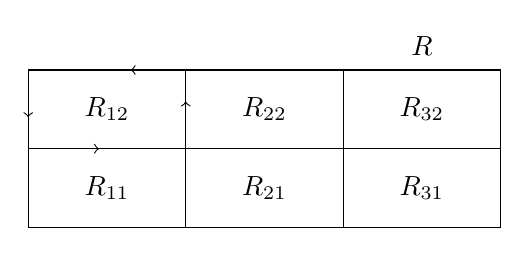
\begin{tikzpicture}
\draw (0,0) rectangle (6,2);
\draw (0,1) -- (6,1);
\draw (2,0) -- (2,2);
\draw (4,0) -- (4,2);
\node at (5,2.3) {$R$};
\node at (1,1.5) {$R_{12}$};
\node at (3,1.5) {$R_{22}$};
\node at (5,1.5) {$R_{32}$};
\node at (1,0.5) {$R_{11}$};
\node at (3,0.5) {$R_{21}$};
\node at (5,0.5) {$R_{31}$};
\draw[->] (1.7,2) -- (1.3,2);
\draw[->] (0,1.8) -- (0,1.4);
\draw[->] (0.4,1) -- (0.9,1);
\draw[->] (2,1.2) -- (2,1.6);
\end{tikzpicture}}

\uline{Exercice :} (de topologie)
justifier en détail le fait que $R$ peut être décomposer en rectangles
$R_{i,j} = A_i \times B_j$ contenu chacun dans un ouvert du sous-recouvrement fini obtenu.

\margin{168}
